\subsection{Analysis}

\begin{figure*}[t]
\subfigure[Default parameters ($R_{AI}=40Mbps$, $K_{max}=200KB$).]
{
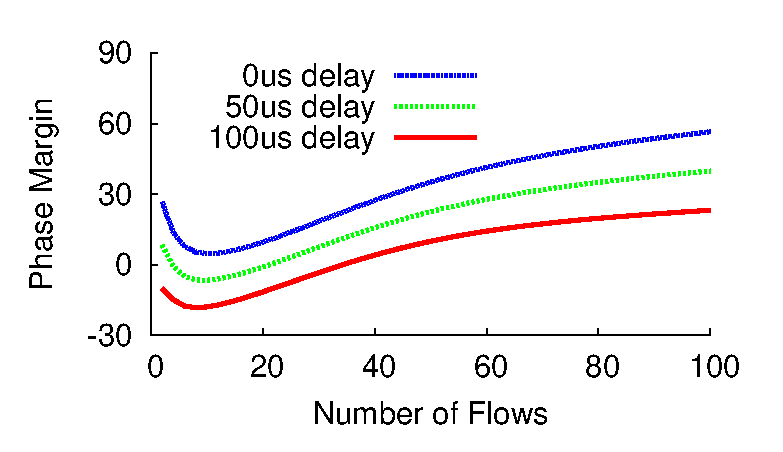
\includegraphics[width=0.33\textwidth]{figures/dcqcn_stability.eps}
\label{fig:dcqcn_stability_default}
}
\subfigure[$R_{AI}=10Mbps$.]
{
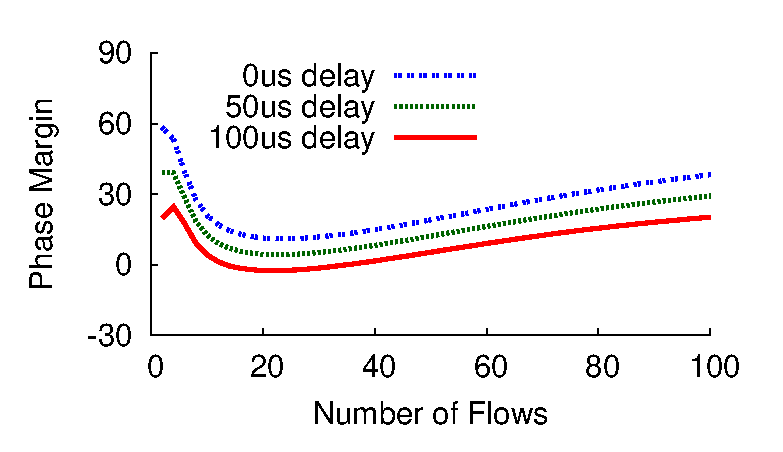
\includegraphics[width=0.33\textwidth]{figures/dcqcn_stability_rai.eps}
\label{fig:dcqcn_stability_rai}
}
\subfigure[$R_{AI}=10Mbps$ and $K_{max}=1000KB$.]
{
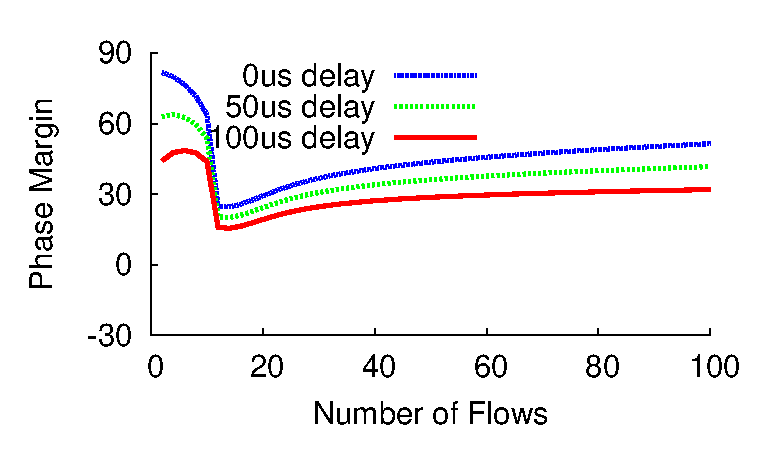
\includegraphics[width=0.33\textwidth]{figures/dcqcn_stability_rai_kmax.eps}
\label{fig:dcqcn_stability_rai_kmax}
}
\caption{DCQCN stability}
\label{fig:dcqcn_stability}
\end{figure*}

Below we show that DCQCN has a unique fixed point at which all flows converged to the 
same rate. We analyze DCQCN's stability around the 
fixed point, how stability varies under different conditions, and conclude with a 
parameter setting guideline.


\para{Fixed point.} By letting the left-hand side of Equation~\ref{eq:q}
be 0, it is easy to see that any of the fixed points (if exist) of DCQCN must satisfy:

\begin{equation}
\small
\sum\limits_{i = 1}^N {R_C^{(i)}(t)} = C
\label{eq:fixedrc}
\end{equation}

At any of the fixed points, we assume the value of $p$ is $p^*$, which is shared by all
flows. The queue length and per-flow
$\alpha^{(i)}$ at the fixed points are determined by Equation~\ref{eq:mark} and \ref{eq:alpha}:

\begin{equation}
\small
{q^*} = \frac{{{p^*}}}{{{p_{max}}}}\left( {{K_{max}} - {K_{min}}} \right) + {K_{min}}
\end{equation}
\begin{equation}
\small
\alpha^{(i)*}  = 1 - {(1 - p^*)^{{\tau '}R_C^{(i)*}}}
\end{equation}

Next, we show that $p^*$ exists and is uniquely determined by $R_C^{(i)*}$ in the DCQCN model. 
From Equation~\ref{eq:rt} and \ref{eq:rc}, at the fixed point, we get the two forms of $R_T^{(i)*}$, respectively:

\begin{equation}
\small
{R_T^{(i)*}} = R_C^{(i)*} + \frac{{a\alpha^{(i)*} }}{{(b + d)\tau }}
\end{equation}
\begin{equation}
\small
{R_T^{(i)*}} = R_C^{(i)*}\left( {1 + \frac{{(c + e)\tau {R_{AI}}}}{a}} \right)
\end{equation}

Where we denote $a, b, c, d, e$ as follows:
\begin{equation}
\begin{array}{l}
a = 1 - {(1 - p^*)^{\tau {R_C^{(i)*}}}},b = \frac{{p^*}}{{{{(1 - p^*)}^{ - B}} - 1}},c = \frac{{{{(1 - p^*)}^{FB}}p^*}}{{{{(1 - p^*)}^{ - B}} - 1}},\\
d = \frac{{p^*}}{{{{(1 - p^*)}^{ - T{R_C^{(i)*}}}} - 1}},e = \frac{{{{(1 - p^*)}^{FT{R_C^{(i)*}}}}p^*}}{{{{(1 - p^*)}^{ - T{R_C^{(i)*}}}} - 1}}
\end{array}
\end{equation}

Combining the two forms of $R_T^{(i)*}$, we see that the value of $p^*$ is determined by:
\begin{equation}
\small
\frac{{{a^2}\alpha^{(i)*} }}{{(b + d)(c + e)}} = {\tau ^2}{R_{AI}}R_C^{(i)*}
\label{eq:p_fixed}
\end{equation}

One can easily find that the left-hand side of the above equation is monotonic when $p \in [0,1]$.
When $p = 0$, the left-hand side of Equation~\ref{eq:p_fixed} is smaller than the right-hand side,
while is vice versa when $p = 1$. Thus DCQCN has a unique fixed point, determined by a unique $p^*$. 
Also, one can easily estimate the value of $p^*$ is very 
close to 0 using numerical approaches. Therefore, we can obtain the taylor series around $p=0$ of the left-hand side:

\begin{equation}
\small
\frac{{{a^2}\alpha }}{{(b + d)(c + e)}} = \frac{{(R_C^{(i)*})^3{\tau ^2}\tau '}}{{{{\left( {\frac{1}{B} + \frac{1}{{TR_C^{(i)*}}}} \right)}^2}}}{p^3} + O\left( {{p^4}} \right)
\end{equation}

Omitting the $O(p^4)$ term, combining Equation~\ref{eq:p_fixed}, we have the fixed point of $p$:

\begin{equation}
\small
{p^*} = \sqrt[3]{{\frac{{{R_{AI}}}}{{{\tau '}(R_C^{(i)*})^2}}{{\left( {\frac{1}{B} + \frac{1}{TR_C^{(i)*}}} \right)}^2}}}
\label{eq:fixedp}
\end{equation}

From the equation above, we see that $p^*$ and $R_C^{(i)*}$ uniquely determine each other. 
Since $p^*$ is shared by any flow $i$, $i = 1, 2, ..., N$, we have:

\begin{equation}
\small
R_C^{(1)*} = R_C^{(2)*} = ... = R_C^{(N)*}
\end{equation}

Combining equation~\ref{eq:fixedrc}, we know that there is only one unique fixed point, at which
$R_C^{(i)*} = \frac{C}{N}$, $i = 1, 2, ..., N$ and $p^*$ is given by equation~\ref{eq:fixedp}.


\para{Stability analysis.} 
We linearize the system by denoting $\delta {R_C}(t) = {R_C}(t) - R_C^*$, $\delta {R_C}(t) = {R_C}(t) - R_C^*$,
$\delta p(t) = p(t) - p^*$, $\delta \alpha (t) = \alpha (t) - \alpha^*$, and $A = \left( {\frac{1}{B} + \frac{1}{{TR_C^*}}} \right)$.
We further use Taylor series to simplify the expressions of $a, b, c, d, e$ to handle the exponential forms like $(1-p)^x$.
Because the equations are very complicated, here we just show an example of $R_C$. The linearized equation of $R_C$ is as follows:

\begin{equation}
\small
\begin{array}{l}
\frac{{d\delta {R_C}}}{{dt}} =  - \frac{1}{2}{(R_C^*)^2}{\alpha ^*}\delta p - \frac{1}{2}{p^*}R_C^*{\alpha ^*}\delta R_C \\
 - \frac{1}{2}{p^*}R_C^*{\alpha ^*}\delta {R_C} - \frac{1}{2}{p^*}{(R_C^*)^2}\delta \alpha \\
 + \frac{A}{2}\left( {R_C^*\delta {R_T} - R_C^*\delta {R_C} + R_T^*\delta {R_C} - R_C^*\delta R_C} \right)\\
 - \left( {\frac{1}{2} + \frac{A}{4}} \right)\left( {{p^*}R_C^*\delta {R_T} - {p^*}R_C^*\delta {R_C} + {p^*}R_T^*\delta {R_C}} \right)\\ 
 - \left( {\frac{1}{2} + \frac{A}{4}} \right)\left( {{p^*}R_C^*\delta R_C - R_C^*R_T^*\delta p + {{(R_C^*)}^2}\delta p} \right)
\end{array}
\end{equation}

We can then perform Laplace transform and get:

\begin{equation}
\small
\begin{array}{l}
s{R_C}(s) - \delta {R_C}(0) = \\
\left( { - \frac{1}{2}{{(R_C^*)}^2}{\alpha ^*} - \left( {\frac{1}{2} + \frac{A}{4}} \right)R_C^*R_T^* + \left( {\frac{1}{2} + \frac{A}{4}} \right){{(R_C^*)}^2}} \right){e^{ - s\tau *}}p(s)\\
 + \left( { - \frac{1}{2}{p^*}R_C^*{\alpha ^*} - \frac{A}{2}R_C^* + \left( {\frac{1}{2} + \frac{A}{4}} \right){p^*}R_C^*} \right){e^{ - s\tau *}}{R_C}(s)\\
 + \left( { - \frac{1}{2}{p^*}R_C^*{\alpha ^*} - \frac{A}{2}R_C^* + \frac{A}{2}R_T^* }\right){R_C}(s)\\
 + \left( { \left( {\frac{1}{2} + \frac{A}{4}} \right){p^*}R_C^* - \left( {\frac{1}{2} + \frac{A}{4}} \right){p^*}R_T^*} \right){R_C}(s)\\
 - \frac{1}{2}{p^*}{(R_C^*)^2}\alpha (s)\\
 + \left( {\frac{A}{2}R_C^* - \left( {\frac{1}{2} + \frac{A}{4}} \right){p^*}R_C^*} \right){R_T}(s)
\end{array}
\end{equation}

With Laplace tranform of the other equations, we can use ${R_C}(s)$ to express ${R_T}(s)$, $p(s)$ and $\alpha (s)$.
Then we can get the characteristic equation of ${R_C}(s)$. We test the characteristic equation against {\em Bode Stability
Criteria}, which is a common methodology in control theory. We show the analysis results in Figure~\ref{fig:dcqcn_stability}. 
The degree of stability is shown as {\em Phase Margin}. The system is stable when its {\em Phase Margin} is larger than 0, 
and the larger {\em Phase Margin} means the system is more stable.

We analyze DCQCN stability in different conditions, particularly with different control signal delays (propagation delay
plus queuing delay in practice), and different number of flows. An ideal protocol should be tolerant with large delay and
scalable to any number of flows. As Figure~\ref{fig:dcqcn_stability} shows, DCQCN, with default parameters, is mostly 
stable. In most cases, the phase margin is larger than 0, while when the delay is large, {\em e.g.,} and with certain 
number of flows, DCQCN may become unstable. The worst stability occurs at around 10 flows. DCQCN is increasingly stable 
with larger number of flows, which means good scalability.

The network operators may tune parameters to make DCQCN more stable. The two most direct parameters are $R_{AI}$ and $K_{max}$.
Smaller $R_{AI}$ means flows increase their rate more gentle, and stabilizes the system. Similarly, larger $K_{max} - K_{min}$
makes rate decreasing more fine grained, because the perturbation of queue length leads to smaller marking probability 
perturbation. We show these trends in Figure~\ref{fig:dcqcn_stability}(b) and (c). With small $R_{AI}$ and large $K_{max}$,
DCQCN can be always stable even when the control signal delay reaches 100$\mu s$, which equals to the propagation delay of a 
$30KM$ cable, or $500KB$ queuing delay. Such large delay is rarely seen in today's datacenter networks.

Here we want to point out that tuning $R_{AI}$ and $K_{max}$ is a trade-off between stability and latency. Smaller $R_{AI}$
makes flows ramp up their rates slower, and larger $K_{max}$ leads to larger queue length. In most cases, the default parameters
strike a good enough balance between stability and latency.

\subsection{Convergence}
